\documentclass[10pt,t,compress]{beamer}

% --------------- Packages ----------------------
% graphics
\usepackage{graphicx}
% Math
\usepackage{amsmath}
\usepackage{amssymb}
\usepackage{amsfonts}
\usepackage{amsthm}
% Color
\usepackage{color}
\usepackage{colortbl}
% Misc
\usepackage{url}
\usepackage{hyperref}
\usepackage[utf8]{inputenc}
\usepackage{xifthen}
\usepackage{bbm}

% ------- tikz -------
\usepackage{tikz}
\usepackage{pgfplots}
\usepackage{tkz-euclide}
\usetikzlibrary{positioning}
\usetikzlibrary{arrows}
\usetikzlibrary{calc}
\usetkzobj{all}
\tikzset{small node/.style={circle,fill=gray!5,draw,minimum size=0.4cm,inner sep=0pt} }
\tikzset{center node/.style={circle,fill=blue!15,draw,minimum size=0.4cm,inner sep=0pt} }
\tikzset{special node/.style={circle,fill=red!20,draw,minimum size=0.4cm,inner sep=0pt} }
\tikzset{final node/.style={circle,fill=green!20,draw,minimum size=0.4cm,inner sep=0pt} }
\tikzset{edge/.style = {->,> = latex, thick, } }
\tikzset{double edge/.style = {<->,> = latex, thick, } }

%---------------- Structure and Themes ----------------
\mode<presentation>
{
    \usefonttheme[onlysmall]{structurebold}
    \usefonttheme[onlymath]{serif}
    \useinnertheme{rectangles}
    \useoutertheme{split}
    %\usecolortheme{orchid}
    \usecolortheme{whale}
}

\setbeamerfont{headline}{size=\Tiny}
\hypersetup{pdfpagemode=UseNone}

%----------------  Color Definition ----------------
\definecolor{UB_Blau_histo}{RGB}{51,153,255}
\definecolor{UB_Blau1}{RGB}{230,235,250}
\definecolor{UB_Blau11}{RGB}{230,235,250}
\definecolor{UB_Blau2}{RGB}{186,204,238}
\definecolor{UB_Blau3}{RGB}{163,189,232}
\definecolor{UB_Blau33}{RGB}{163,189,232}
\definecolor{UB_green}{RGB}{251,255,251}
\definecolor{midgreen}{RGB}{60,200,20}
\definecolor{lightgreen}{RGB}{190,247,175}
\definecolor{lightyellow}{RGB}{255,255,147}
\definecolor{weiss}{RGB}{255,255,255}
\definecolor{grau}{gray}{.90}
\definecolor{blue1}{rgb}{0.32,0.93,0.91}
\definecolor{blue2}{rgb}{0.18,0.59,1.00}
\definecolor{lightblue2}{rgb}{0.85,0.85,1.00}
\definecolor{lightgreen}{rgb}{0.80,1.00,0.80}
\definecolor{lightblue1}{rgb}{0.80,1.00,1.00}
\definecolor{green2}{rgb}{1.00,1.00,0.00}

\definecolor{col1}{RGB}{0,255,0}
\definecolor{col2}{RGB}{102,204,0}
\definecolor{col3}{RGB}{255,255,0}
\definecolor{col4}{RGB}{255,128,0}
\definecolor{col5}{RGB}{255,0,0}

\setbeamercolor*{palette primary}{use=structure,fg=black,bg=UB_Blau1!}
\setbeamercolor*{palette secondary}{use=structure,fg=white,bg=structure.fg!75!black}
\setbeamercolor*{palette tertiary}{use=structure,fg=white,bg=structure.fg!50!black}
\setbeamercolor*{palette quaternary}{fg=black,bg=white}

\setbeamercolor{block title}{use=structure,fg=black,bg=UB_Blau33}
\setbeamercolor{block body}{parent=normal text,use=block title,bg=UB_Blau11}

\setbeamercolor{block body example}{parent=normal text,use=block title,bg=UB_green}

\setbeamercolor{section in head/foot}{parent=palette quaternary}
\setbeamercolor{subsection in head/foot}{parent=palette quaternary}

\setbeamercolor{author in head/foot}{parent=palette primary}
\setbeamercolor{title in head/foot}{parent=palette primary}

% ------- Fix width headline (split)w/ sections w/o subsections --------------
\makeatletter
\setbeamertemplate{headline}
{%
	\leavevmode%
	\begin{beamercolorbox}[wd=\paperwidth,ht=2.5ex,dp=1.125ex]{section in head/foot}%
		\insertsectionnavigationhorizontal{.5\paperwidth}{\hskip0pt plus1filll}{}%
	\end{beamercolorbox}%
}
\makeatother

%----------------  Seitenzahlen ----------------
\defbeamertemplate*{slidenumber}{framenumber} {\insertframenumber}
\defbeamertemplate{slidenumber}{totalframenumber} {\insertframenumber\,/\,\inserttotalframenumber}
\defbeamertemplate{slidenumber}{pagenumber} {\insertpagenumber}
\defbeamertemplate{slidenumber}{totalpagenumber} {\insertpagenumber\,/\,\insertpresentationendpage}

\setbeamertemplate{navigation symbols}{}

\defbeamertemplate*{footline}{slidenumber right}
{
  \leavevmode
  \hbox{\begin{beamercolorbox}[wd=\paperwidth,ht=2.5ex,dp=1.125ex,leftskip=.3cm,rightskip=.3cm]{title in head/foot}
    \usebeamerfont{title in head/foot}
    \insertshorttitle \hfill \insertshortauthor \hfill \usebeamertemplate{slidenumber}
  \end{beamercolorbox}}
}

% Set notation
\newcommand{\E}[1]{\mathbb{E}\left[#1\right]}
\newcommand{\dist}[1]{\left\|#1\right\|}
\newcommand{\ctr}[1]{\text{ctr}\left(#1\right)}
\newcommand{\real}{\mathbb{R}}
\newcommand{\realp}{\mathbb{R}_{+}}
\newcommand{\realzp}{\mathbb{R}_{\ge 0}}
\newcommand{\integer}{\mathbb{Z}}
\newcommand{\integerp}{\mathbb{Z}_{>0}}
\newcommand{\integerzp}{\mathbb{Z}_{\ge 0}}
\newcommand{\argmin}{\mathrm{arg\,min}}

\newcommand{\explain}[2]{\underset{\mathclap{\overset{\uparrow}{#2}}}{#1}}
\newcommand{\explainup}[2]{\overset{\mathclap{\underset{\downarrow}{#2}}}{#1}}


\setbeamercovered{invisible}

%Logo Position upper right
	\pgfdeclareimage[height=0.5cm]{uni}{./Images/logo4.pdf}
\logo{\pgfuseimage{uni}}

\makeatletter
\setbeamertemplate{frametitle}{%
  \begin{beamercolorbox}[wd=\paperwidth,leftskip=.5cm,% von links her eingeschoben
       rightskip=-1mm,vmode,sep=0.0001cm]{frametitle}
%  \begin{beamercolorbox}[sep=0.3cm,#1,wd=\the\@tempdima]{frametitle}
    \usebeamerfont*{frametitle}%
        %\vbox{}%\vskip-0ex%
    \strut\insertframetitle\strut\hfill\parbox{1.8cm}{\insertlogo}% xx cm nach links eingeschoben
      \ifx\insertframesubtitle\@empty\else\par%
        {\usebeamerfont*{framesubtitle}{%
         \usebeamercolor[fg]{framesubtitle}%
         \insertframesubtitle}\strut\par}%
      \fi%
  \end{beamercolorbox}}
\makeatother
\setbeamertemplate{sidebar right}{% hier kein logo
  \vfill%
  \vskip2pt%
  \llap{\usebeamertemplate***{navigation symbols}\hskip0.1cm}%
  \vskip2pt%
}

% ---- Fix citations ---
\setbeamertemplate{bibliography item}{}

% ---- List settings ---
\setlength\itemsep{0pt}
\setlength{\parskip}{0pt}

% --------- Show Notes (yes or no) --------------
\setbeameroption{hide notes}% {hide, show, show only}
\setbeamertemplate{note page}[compress]
\setbeamerfont{note page}{size=\footnotesize}

% -----------Theorems ---------------------------
\newtheorem{defn}{Definition}
\newtheorem{alg}{Algorithm}
\newtheorem{lem}{Lemma}
\newtheorem{thm}{Theorem}

% --------- Presentation Details ----------------
\thispagestyle{empty}

\title[Convex Relaxations for CSP]{Convex Relaxations for Constraint Satisfaction Problems}

\author{Raaz Dwivedi, Riley Murray, Quico Spaen}
\institute{University of California, Berkeley}

\date{EE227B Project\\ December 1, 2015}

\setlength{\unitlength}{1mm}

\begin{document}

% --- Title page ---
\frame{\titlepage}

\section{Constraint Satisfaction Problem}

\begin{frame}{Constraint Satisfaction Problem}
	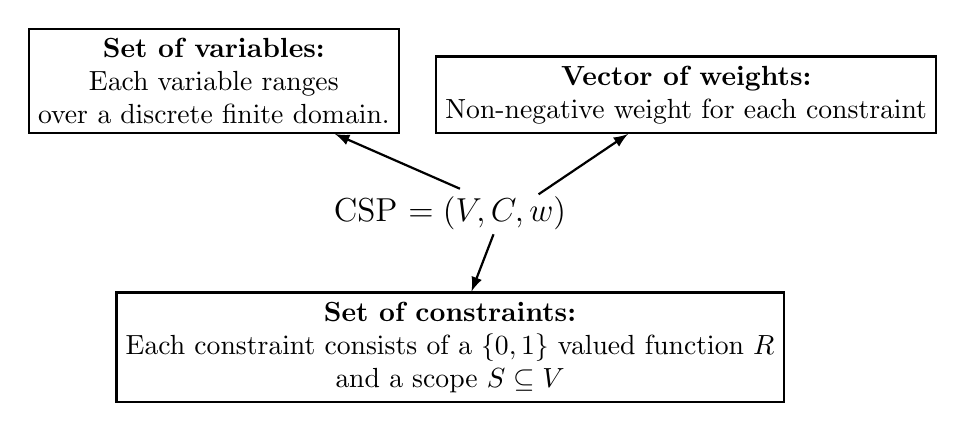
\begin{tikzpicture}
	\node[] (CSP) at (0,0) {\large CSP $ = (V,C,w)$};
	\node[] (CSPv) at (.25,.25) {};
	\node[] (CSPc) at (.60,-.15) {};
	\node[] (CSPw) at (1,.15) {};
	\visible<2->{
	\node[draw, thick, rectangle, align=center, anchor= south] (variables) at (-3,1) {{\bf Set of variables:}\\ Each variable ranges\\ over a discrete finite domain.};
	\draw[edge] (CSPv) to (variables);
	}
	\visible<3->{
	\node[draw, thick, rectangle, align=center, anchor= north] (constraints) at (0,-1) {{\bf Set of constraints:}\\ Each constraint consists of a $\{0,1\}$ valued function $R$\\ and a scope $S \subseteq V$};
	\draw[edge] (CSPc) to (constraints);
	}
	\visible<4->{
		\node[draw, thick, rectangle, align=center, anchor= south] (weights) at (3,1) {{\bf Vector of weights:}\\ Non-negative weight for each constraint};
		\draw[edge] (CSPw) to (weights);
	}

	\end{tikzpicture}\\
	\pause[5]
	\begin{block}{Objective}
		Maximize weighted sum of satisfied constraints
	\end{block}
	\pause
	Examples:
	\begin{itemize}
		\item SAT: Constraints of the form $ x_1 \vee \bar{x}_4 \vee x_7 $, $x_i \in \{0,1\}$
		\item Max-Cut
	\end{itemize}
\end{frame}

% -------- LP -----------
\section{LP Relaxation}

\begin{frame}{LP Relaxation}
\begin{block}{Idea}
Formulate the CSP as an integer program (the equivalent formulation is exact and hence NP-hard) by introducing dummy $\{ 0, 1\}$-valued variables (indicators) for each variable and each constraint \pause \emph{ and then relax it to get an LP.}
\end{block}
\pause
 For each variable $i \in V$, we define
 \[
	 \mu_i[\ell] = \mathbbm{1}( \text{variable $i$ takes value } \ell)
 \] 
\pause  Similarly, for each constraint $j \in C$,
   \[
   \lambda_j[L] = \mathbbm{1}( \text{assignment $L$ is chosen for constraint $j$})
   \] 
\pause
We impose two consistency conditions 
 \begin{itemize}
 \item $\displaystyle\sum_{\ell \in D} \mu_i[\ell] = 1$, $\displaystyle\sum_{L} \lambda_j[L] = 1$ $\Rightarrow$ exactly one indicator is non-zero.
 \pause
 \item $\mu_i[\ell] = \displaystyle\sum_{L(i) = \ell} \lambda_j[L] \Rightarrow$ Consistency in assignments
 \end{itemize}
\pause Relax $\mu_i[\ell] \in \{ 0, 1\} \rightarrow \mu_i[\ell] \in [0, 1]$ and $\lambda_j[L] \in \{ 0, 1\} \rightarrow \lambda_j[L] \in [0, 1]$.

\end{frame}

% -------- SDP -----------
\section{SDP Relaxation}


\begin{frame}{An SDP Relaxation}
\begin{block}{Idea}
\begin{itemize}
\item The LP formulation has no information on \textit{joint} distributions of variables. This information could be valuable!
\item Find a joint distribution by introducing a \textbf{covariance matrix}.
\end{itemize}
\end{block}
\textit{Build} on the LP : introduce  ``$X_{(i,\ell),(i',\ell')}$" with interpretation
$$X_{(i,\ell),(i',\ell')} = \text{Pr}\left( \hat{L}_j(i) = \ell \text{ and } \hat{L}_j(i') = \ell'\right)
 $$
$ \text{ where } \hat{L}_j = L  \text{ w.p. } \lambda_j\left[L\right]$. Enforce this interpretation with
\begin{align*}
 \text{(LMI) } X \succeq 0  \quad & \text{ (Affine)} \quad X_{(i,\ell),(i,\ell')} = 0  \quad  \forall ~  \ell \neq \ell' \\
 \text{ and } &\text{ (Affine)} \quad \textstyle{\sum_{L \in \mathcal{L}_j \wedge L(i) = \ell \wedge L(i') = \ell'}} \lambda_j\left[L\right] = X_{(i,\ell),(i',\ell')}
\end{align*}
Solve this SDP to get covariance matrix $X$. Now how do we use it?
\end{frame}

% -------- Rounding -----------
\section{Rounding}
\begin{frame}{Rounding Schemes}
Given the solution of relaxations, we need to find a good assignment.
\pause
\begin{block}{Rounding LP}
For LP, we have a probability mass function $\mu_i[\cdot]$ for each variable. \pause We can generate random numbers "independently" for each variable according to these pmf's and assign it to the variable to get an assignment. \pause Is it good enough? \pause We have (for MAX-SAT)
\[\small \mathbb{E}[\mbox{LP Rounding}] \geq \left(1-\frac{1}{e} \right) \mbox{Opt}(C) \]
\end{block}

\pause
\begin{block}{SDP Rounding}
The random variables are no longer independent and hence we need to generate "dependent" set of random numbers whose covariance matrix is related to $X$.
\end{block}
\end{frame}
\end{document}
